%  Document Config
\documentclass[12pt]{diazessay}



\ksulogo{
    \begin{tikzpicture}[remember picture,overlay]
    \node[anchor=north west,yshift=-1.5pt,xshift=1pt]%
        at (current page.north west)
        {
\includegraphics[height=30mm]{Figures/KSU_logo.png}};
    \end{tikzpicture}
}

\school{King Saud University \\
College of Computer and Information Sciences\\
Computer Science Department}

\title{\textbf{Arabic Text Dialect Recognition}}

\logo{
    \begin{figure}[h]
        % \hskip-3.3cm
        \centering
        
\includegraphics[scale=0.2]{Figures/best_project_logo.png}
    \end{figure}
}

\author{\textbf{Authors} \\ 
Mohand Al-Rasheed \hspace{15pt} 439101298\\
Khalid Albader \hspace{50pt}  439101990\\
Abdulrahman Alshawi \hspace{4pt}  439101980\\
Abdullah Alsuwailem \hspace{11pt}  439101690\\
Musaad Alqubayl \hspace{35pt}  439101884\\
} 
\supervisor{Dr. Nasser Alsadhan}

\date{Research project for the degree of Bachelor in Computer Science \\
First/Second Semester 1443 \\
Autumn/Spring 2021}

% Image config
\usepackage{graphicx}
\graphicspath{ {./Figures/} }

% Code config
\usepackage{listings}
\usepackage{color}

\definecolor{dkgreen}{rgb}{0,0.6,0}
\definecolor{gray}{rgb}{0.5,0.5,0.5}
\definecolor{mauve}{rgb}{0.58,0,0.82}
\definecolor{backcolour}{rgb}{0.99,0.99,0.99}


\lstset{frame=tb,
  language=Python,
  aboveskip=3mm,
  belowskip=3mm,
  showstringspaces=false,
  columns=flexible,
  basicstyle={\small\ttfamily},
  backgroundcolor=\color{backcolour},   
  numbers=left,
  numberstyle=\tiny\color{gray},
  keywordstyle=\color{blue},
  commentstyle=\color{dkgreen},
  stringstyle=\color{mauve},
  breaklines=True,
  breakatwhitespace=true,
  tabsize=1
}


% Section config
\usepackage{titlesec}
\usepackage{hyperref}

\titleclass{\subsubsubsection}{straight}[\subsection]

\newcounter{subsubsubsection}[subsubsection]
\renewcommand\thesubsubsubsection{\thesubsubsection.\arabic{subsubsubsection}}
\renewcommand\theparagraph{\thesubsubsubsection.\arabic{paragraph}} % optional; useful if paragraphs are to be numbered

\titleformat{\subsubsubsection}
  {\normalfont\normalsize\bfseries}{\thesubsubsubsection}{1em}{}
\titlespacing*{\subsubsubsection}
{0pt}{3.25ex plus 1ex minus .2ex}{1.5ex plus .2ex}

\makeatletter
\renewcommand\paragraph{\@startsection{paragraph}{5}{\z@}%
  {3.25ex \@plus1ex \@minus.2ex}%
  {-1em}%
  {\normalfont\normalsize\bfseries}}
\renewcommand\subparagraph{\@startsection{subparagraph}{6}{\parindent}%
  {3.25ex \@plus1ex \@minus .2ex}%
  {-1em}%
  {\normalfont\normalsize\bfseries}}
\def\toclevel@subsubsubsection{4}
\def\toclevel@paragraph{5}
\def\toclevel@paragraph{6}
\def\l@subsubsubsection{\@dottedtocline{4}{7em}{4em}}
\def\l@paragraph{\@dottedtocline{5}{10em}{5em}}
\def\l@subparagraph{\@dottedtocline{6}{14em}{6em}}
\makeatother

\setcounter{secnumdepth}{4}
\setcounter{tocdepth}{4}


\begin{document}


\maketitle 


%----------------------------------------------------------------------------------------
%	ESSAY BODY
%----------------------------------------------------------------------------------------

\tableofcontents

\cleardoublepage

\addcontentsline{toc}{section}{Acknowledgements}
\section*{Acknowledgements}
We would like to express our great gratitude to Dr. Nasser Alsadhan for his valuable suggestions. and his aid throughout the writing of this report. His willingness to give his time so generously has been very much appreciated.

\addcontentsline{toc}{section}{English Abstract}
\section*{English Abstract}
The Arabic language is one of the oldest languages widely used today, and as a result of that, many Arabic speaking regions have formed dialects exclusive to their own. For example, many countries surrounding the Arabic Gulf have formed a dialect different to countries in the Levantine region. We intend on identifying and systematically determining the dialect of a piece of text. 

 This research has many applications in Arabic text analysis, such as helping in identifying the regions customers most often come from by analyzing a product’s reviews and comments and breaking them down by region, which provides useful intel for a business. It also helps in narrowing the nationality of an anonymous writer of a piece of text by predicting their region.
One of the major challenges in dialect recognition is dividing data into classes of dialects. Saudi Arabia and the UAE have dialects that differ widely from each other when solely considered, though they feel very similar in comparison to a Levantine dialect. The researchers will determine a classification easy enough for a machine to detect, but sophisticated enough to be useful. 

We intend to build a machine learning powered classifier that distinguishes between a set number of different Arabic dialects (e.g. Egyptian, Levantine, Gulf, etc.) when given a piece of text. We’ll use state of the art technologies in the field of NLP (natural language processing) in order to train an effective classifier that understands the differences between dialects.


\addcontentsline{toc}{section}{Arabic Abstract}
\section*{Arabic Abstract}
\begin{RLtext}
اللغة العربية من أقدم اللغات المستخدمة بكثرة حاليا، ونتيجة لذلك، الكثير من المناطق المتحدثة للعربية أنشأت لهجات مخصصة بمناطقهم. فعلى سبيل المثال، الكثير من المناطق المجاورة للخليج العربي تتحدث لهجة مختلفة بشدة عن لهجات المناطق الشامية. يعتزم الباحثون على أتمتة عملية التعرف على اللهجات من خلال تحليل قطعة من النص.

البحث له العديد من التطبيقات، وأهمها هو في تحليل النصوص العربية، فمثلا استخدامه في التعرف على مناطق عملاء جهة معينة عن طريق تحليل التقاييم والتعليقات المضافة على منتجاتهم، مما يمكن الجهة على التعرف على عملائهم بشكل أدق. كذلك يمكن استخدامه للتنبؤ بمنشأ مرسل رسالة مجهولة عن طريق التعرف على منطقة انتمائه.

من أهم التحديات في تصنيف اللهجات هي تقسيم البيانات لأصناف من اللهجات. فعلى سبيل المثال، المملكة العربية السعودية والإمارات العربية المتحدة يتحدثون بلهجات مختلفة إذا حصرنا النظر عليهم، ولكن يشبهون بعض حين تتم مقارنتهم مع اللهجات الشامية. سيختار الباحثون مجموعة مناسبة من اللهجات حيث تكون سهلة للنظام في التعرف عليها، ولكن معقدة كفاية لكي تكون مفيدة.

في هذا المشروع ننوي بناء مصنف (\LR{classifier}) مدعوم بتقنيات تعلم الآلة لكي يصنف ما بين مجموعة من اللهجات المحددة (مثل اللهجة المصرية، والشامية، والخليجية، وغيرها) إذا أعطي قطعة من النص. سيستخدم الباحثون أحدث التقنيات في مجال تحليل اللغات الطبيعية (\LR{NLP}) لكي يدربوا مصنف فعال، يفرق بين اللهجات العربية.
\end{RLtext}


\section{Introduction}
    %link for referenced sentence (Every individual ...) https://dl.acm.org/doi/book/10.5555/2126240
    A dialect is the variation of a language in grammar, pronunciation and vocabulary. Every individual has their own way of talking that is affected by dialect, accent, background and many other factors\cite{10.5555/2126240}. The Arabic language has a variety of dialects throughout the Arabic world, dialects could differ not only across countries but also in the same country or even city. Arabic dialects differ from one another in pronunciation and vocabulary, different dialects have different words or different variations of a word that could refer to the same meaning, which sometimes make it a bit difficult to understand each other, and it can make it harder for non-Arabic speakers who are trying to learn Arabic.
    
    % Link for definition https://www.ibm.com/cloud/learn/machine-learning
    Machine learning is a branch of artificial intelligence (AI) and computer science which focuses on the use of data and algorithms to imitate the way that humans learn, gradually improving its accuracy\cite{ibm_cloud_education_2020}. It is a rapidly growing field, many countries are racing each other to adapt machine learning technologies and develop smart and automated systems, applications, and adapt them into our daily lives as well as numerous varieties of fields that could benefit from them. Natural language processing, abbreviated as \textit{NLP} is a branch of machine learning that is primarily focused on analyzing text. Numerous companies are racing to develop programs that utilize NLP to analyze user behaviour. One of the difficulties facing companies developing using NLP for Arabic speakers is the numerous varieties of dialects in Arabic. 
    
    As each language has numerous dialects across regions, researchers became interested in dialect recognition since it is related to more insightful text analysis.


    \subsection{Problem statement}
    
    Dialects are formed mainly due to regional disconnection between the Arab world. This disconnection separates Arab people and reduces the friction between them, and as a result of that, many Arabic speaking regions have formed dialects exclusive to their own. For example, many countries surrounding the Arabic Gulf have formed a dialect different to countries in the Levantine region. The research’s main problem is how to identify and predict dialect types from written text.

 
    \begin{figure}[h]
        % \hskip-3.3cm
        \centering
        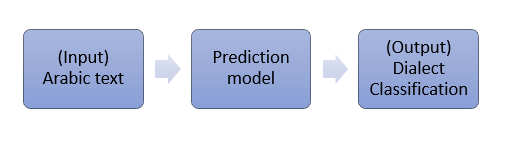
\includegraphics[scale=0.7]{Figures/problem_statment.png}
        \caption{Illustration of the problem}
        \label{fig:cmp}
    \end{figure}
        
    
    \subsection{Goals and objectives}
    
    The goal of this research is to analyze and an Arabic text to classify the dialect of the given text.
    The objective is to build upon the Arabic corpora collected by older researches on this topic and to implement the most appropriate state of the art NLP model that helps in achieving the best possible accuracy which correlates to correctly classifying what dialect the text is from. As well as enrich the existing Arabic corpora by collect text from many different dialects.

    \subsection{Proposed Solution}
    
    This research will contribute in solving Arabic dialect detection by using one of the latest advancements in the field of natural language processing while also gathering more Arabic dialect text on top of the existing corpora when necessary.
    
    \subsection{Research scope}
    
    The scope of this research is mainly focused about gathering (when needed), preprocessing and modeling state of the art NLP to classify Arabic text. 

\section{Background}

    \subsection{Natural language processing}
    
    \subsection{Preprocessing}

    \subsection{Dialect prediction approaches}
    
        \subsubsection{Approach 1}
        \subsubsection{Approach 2}
        \subsubsection{Approach 3}



\bibliographystyle{plain} % We choose the &quot;plain&quot; reference style
\bibliography{cite.bib} % Entries are in the &quot;refs.bib&quot; file</code></pre>

\end{document}
